The observations consist of two parts: the VTOL drone's state (body orientation, as well as the translational and rotational velocities) and the relative path to the next two waypoints. The observation vector is denoted as  $o(t) = \left[R_W(t), v_B(t), \omega_B(t), wp_B(t), nwp_B(t)\right],$ where $R_W(t)$, $v_B(t)$, $\omega_B(t)$, are the drone's rotation matrix, velocity, body rates and $wp_B(t)$, $nwp_B(t)$ are the relative path to the next two waypoints of the trajectory. The action vector produced by the policy $a(t) = \left[f_1,f_2,f_3,f_4\right]$ gives the PWM signals for each rotor individually. In Figure \ref{fig:actor} both observation and action space are illustrated, as well as the actor network architecture, which is a 2-layer multilayer perceptron (MLP). For more details on the network architecture see Section \ref{subsec:training_details}.

\begin{figure*}[h]
\centering
\begin{subfigure}[ht]{0.45\textwidth}
    \centering
    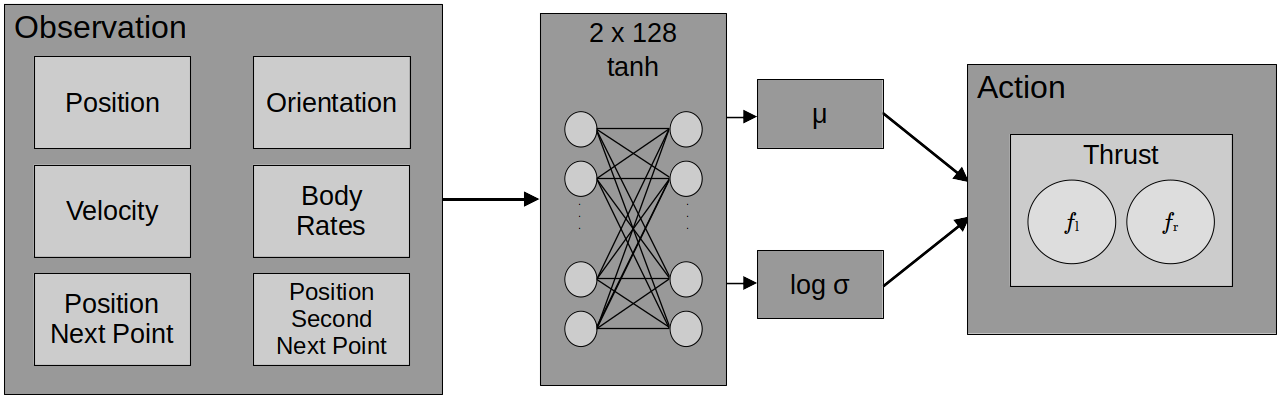
\includegraphics[width=1.0\textwidth]{images/2Dactor_short.png}
    \caption{Actor network for elektra VTOL3 controller in 2D world.}
    \label{fig:actor_2D}
\end{subfigure}
\hfill
\begin{subfigure}[h]{0.45\textwidth}
    \centering
    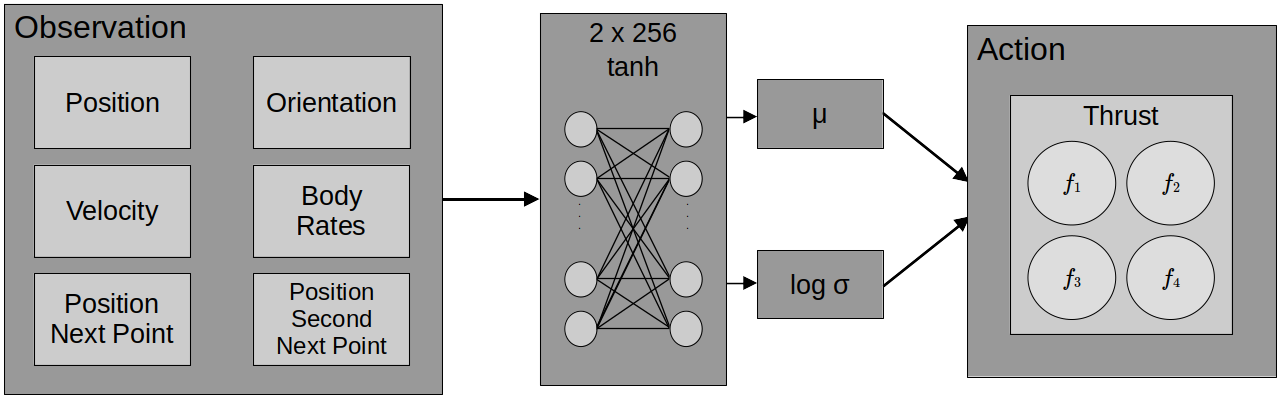
\includegraphics[width=1.0\textwidth]{images/3Dactor_short.png}
    \caption{Actor network for quadrotor controller in 3D world.}
    \label{fig:actor_2D}
\end{subfigure}
\caption{Illustration of the actor networks with the used observation and action spaces.}
\label{fig:actor}
\end{figure*}